% -*- TeX:de -*-
\NeedsTeXFormat{LaTeX2e}
\documentclass[12pt,a4paper]{article}
\usepackage[german]{babel} % german text
\usepackage[DIV12]{typearea} % size of printable area
\usepackage[T1]{fontenc} % font encoding
%\usepackage[latin1]{inputenc} % most likely on Windows
\usepackage[utf8]{inputenc} % probably on Linux
\usepackage{multicol}

% PLOTTING
\usepackage{pgfplots} 
\usepackage{pgfplotstable}
\usepackage{url}
\usepackage{graphicx} % to include images
\usepackage{tikz}
\usepackage{subfigure} % for creating subfigures
\usepackage{amsmath} % a bunch of symbols
\usepackage{amssymb} % even more symbols
\usepackage{booktabs} % pretty tables
\usepackage{makecell} % multi row table heading

% a floating environment for circuits
\usepackage{float}
\usepackage{caption}

%\newfloat{circuit}{tbph}{circuits}
%\floatname{circuit}{Schaltplan}

% a floating environment for diagrams
%\newfloat{diagram}{tbph}{diagrams}
%\floatname{diagram}{Diagramm}

\selectlanguage{german} % use german

\begin{document}








%%%% TO DO
%
% - - Shorty:
%
% - - Tabelle "Messwerte Linsenbrennweite"
%		bitte bei jedem neuen e eine trennlinie... bin zu deppert ^^

% - - Patrick
%




%%%%%%% DECKBLATT %%%%%%%
\thispagestyle{empty}
			\begin{center}
			\Large{Fakultät für Physik}\\
			\end{center}
\begin{verbatim}


\end{verbatim}
							%Eintrag des Wintersemesters
			\begin{center}
			\textbf{\LARGE WS 2013/14}
			\end{center}
\begin{verbatim}


\end{verbatim}
			\begin{center}
			\textbf{\LARGE{Physikalisches Praktikum\\ für das Bachelorstudium}}
			\end{center}
\begin{verbatim}




\end{verbatim}

			\begin{center}
			\textbf{\LARGE{PROTOKOLL}}
			\end{center}
			
\begin{verbatim}





\end{verbatim}

			\begin{flushleft}
			\textbf{\Large{Experiment (Nr., Titel):}}\\
							%Experiment Nr. und Titel statt den Punkten eintragen
			\LARGE{PW6 Geometrische Optik}	
			\end{flushleft}

\begin{verbatim}

\end{verbatim}	
							%Eintragen des Abgabedatums, oder des Erstelldatums des Protokolls
			\begin{flushleft}
			\textbf{\Large{Datum:}} \Large{14.11.2013}
			\end{flushleft}
			
\begin{verbatim}
\end{verbatim}
							%Namen der Protokollschreiber
		\begin{flushleft}
			\textbf{\Large{Namen:}} \Large{Patrick Braun, Johannes Kurz}
			\end{flushleft}

\begin{verbatim}


\end{verbatim}
							%Kurstag und Gruppennummer, zb. Fr/5
			\begin{flushleft}
			\textbf{\Large{Kurstag/Gruppe:}} \Large{DO/2}
			\end{flushleft}

\begin{verbatim}



\end{verbatim}
							%Name des Betreuers, das Praktikum betreute.
			\begin{flushleft}
			\LARGE{\textbf{Betreuer:}}	\Large{ Johanna Akbarzadeh }	
			\end{flushleft}

%%%%%%% DECKBLATT ENDE %%%%%%%
\pagebreak
\setlength{\columnsep}{20pt}
\begin{multicols}{2}

%%%%%%%%%%%%%%%%%%%%%%%%%%%%%%%%%%%%
\section{Brennweite von Linsen}
Die \textbf{Brennweite $f $} einer Linse ist der Abstand zwischen Brennpunkt und der angenommenen Brechungsebene einer Linse. \\
Für Sammellinsen (konvexe) gehen (idealerweise) alle parallel zur optischen Achse einfallenden Strahlen durch den Brennpunkt.\\
Für Konkave Linsen, die Parallelstrahlen so brechen, dass sie auseinanderstreuen, liegt ein imaginärer Brennpunkt vor der Linse, in welchem die Verlängerungen der Strahlen gebündelt sind. Daher haben die Brennweiten von Zerstreuungslinsen ein negatives Vorzeichen.\\
\\
In diesem Beispiel soll die Brennweite von einer Konkav- und einer Konvexlinse bestimmt werden.\\
Durch geometrische Überlegungen, aus der Abbildung eines Gegenstands durch eine Linse (\textbf{Gegenstandsweite $g$}, \textbf{Bildweite $b$}) lässt sich, anhand der 3 Hauptstrahlen die Abbildungsgleichung für Linsen herleiten:
$$\frac{1}{f}=\frac{1}{g}+ \frac{1}{b}$$
Zur Bestimmung wird ein Gegenstand (hier eine Schablone) durch eine Linse auf einen Abbildungsschirm scharf gestellt. Durch mehrmalige Messung der Gegenstands- und Bildweite, wird also die Brennweite einer Konvexlinse bestimmt.\\
Eine zweite in diesem Versuch angewandte Methode ist das Besselverfahren:\\
Es wird dabei ausgenutzt, dass bei festem \textbf{Abstand $e$} zwischen Gegenstand und Bild, an 2 Positionen der Linse ein scharfe Abbildung gegeben ist (jedenfalls $e > 4\cdot f$).\\
$d =$ $Abstand$ $zwischen$ $beiden$ $Positionen$
$e=$ $Abstand$ $Gegenstand-Schirm$\\
\\
Aus der Beziehung $e = g + b$ und $d=|g-b|$ lässt sich durch Umformungen aus der Abbildungsgleichung erhalten:
$$f=\frac{1}{4} \left(e-\frac{d^2}{e} \right)$$
\\
Zuletzt soll die Brennweite einer Konkavlinse bestimmt werden.\\
Da diese kein reelles Bild liefert, wird sie zur Messung gemeinsam mit der zuvor vermessenen Konvexlinse auf den Lichtstrahl angewendet. Nachdem das Bild scharf gestellt wurde, lässt sich die Bildweite, jedoch nicht die Gegenstandsweite direkt messen. Diese ergibt sich (in Kenntnis der zuvor gemessenen Bildweite der konvexen) durch
$$g_{konkav}= -(b_{konvex}-d_{konv-konk})$$


\subsection{Messwerte und Ergebnisse}



\begin{figure}[H]
	\centering
	\pgfplotstabletypeset[
			columns={e,g1,g2},
			col sep=&,
			columns/e/.style={column name=\makecell{$e$\\$[cm]$}, precision=1, zerofill}, %
			columns/g1/.style={column name=\makecell{$g1$\\$[cm]$}, precision=1, zerofill},
			columns/g2/.style={column name=\makecell{$g2$\\$[cm]$}, precision=1, zerofill},
			every head row/.style={before row=\hline,after row=\hline\hline},
			every last row/.style={after row=\hline},
			every first column/.style={
								column type/.add={|}{}
							        },
			every last column/.style={
								column type/.add={}{|}
								}
			]{
			e & g1 & g2
			40 & 17.5 & 22.8
			      & 17.3 & 22.5
			      & 17.2 & 23.5
			      & 17.5 & 23.5
			      & 17.5 & 23.0
			
			50 & 13.4 & 36.8
			      & 13.3 & 36.7
			45 & 14.5 & 30.6
			      & 14.5 & 30.7
			60 &  12.4 & 47.8
			65 & 12.0 & 53.0
			}
	\caption{Je 2 Gegenstandsweiten bei verschiedenen Schirmabständen - Konvexlinse}
	\label{fig:Gegenstandsweiten_Konvexlinse}
\end{figure}

\begin{itemize}
	\item $e = (40.0 \pm 0.1) cm$\\
	$g_1 = (17.4 \pm 0.1)cm$\\
	$g_2 =(23.1 \pm 0.2) cm$\\
	\\
	$$f_{G/B}=(9.831\pm 0.023) cm$$
	$$\widehat{=}(0.10172 \pm 0.00024)Dioptrien$$
	$$f_{Bessel} = (9.797 \pm 0.031)cm$$
	
	
	\item $e = (50.0 \pm 0.1)cm$\\
	\indent $g_1 = (13.4 \pm 0.2) cm$\\
	$g_2 = (36.8 \pm 0.2)cm$
	$$f_{Bessel} = (9.762 \pm 0.099) cm$$
	
	\item $e= (45.0 \pm 0.1)cm$\\
	\indent $g_1 = (14.5 \pm 0.2) cm$\\
	$g_2 = (30.6 \pm 0.2) cm$
	$$f_{Bessel}=(9.810 \pm 0.049cm)$$
	
	\item $e=(60.0 \pm 0.1)cm$\\
	\indent $g_1= (12.4 \pm 0.2) cm$\\
	$g_2 = (47.8 \pm 0.2)cm$
	$$f_{Bessel}=(9.78 \pm 0.13) cm$$
	
	\item $e=(65.0 \pm 0.1)cm$\\
	\indent $g_1 = (12.0 \pm 0.2) cm$\\
	$g_2 =(53.0 \pm 0.2)cm$
	$$f_{Bessel} = (9.78 \pm 0.14)cm$$

\end{itemize}

\textbf{Mittel aller 5 Besselmessungen:}\\
$$f=(9.786 \pm 0.045)$$
$$Brechkraft: (0.10219 \pm 0.00047) Dioptrien$$\\
\\
\textbf{Konkavlinse:}
\begin{itemize}
	\item $b_{konvex}=(14.4 \pm 0.2) cm$\\
	$b_{konkav}=(16.7 \pm 0.2)cm$\\
	$d=(8.4 \pm 0.1)cm$
	$$f_{konkav}= (-9.36 \pm 0.70)cm$$
	$$\widehat{=}(-0.10684 \pm 0.00052)Dioptrien$$
	
	\item $b_{konvex}=(17.2 \pm 0.2)cm$\\
	$b_{konvex}=(59.2 \pm 0.4)cm$\\
	$d=(9.2 \pm 0.1)cm$
	$$f_{konkav}= (-9.25 \pm 0.30)cm$$
	$$\widehat{=}(-0.10811 \pm 0.00036)Dioptrien$$
	
	
\end{itemize}




\subsection{Diskussion}
Aus der Messreihe der Gegenstandsweite für $e=40.0cm$ wurde der erste gemessene Wert für $g_1$ entfernt. Dieser wurde erhalten, noch bevor das Licht im Raum gedimmt wurde und eine geeignete Arbeitsweise zum Scharfstellen der Abbildungen gefunden wurde. Daher darf der Messwert, der mit $g_1 = 16.7 cm$ deutlich niedriger als alle 5 anderen ist, als falsch angesehen werden(Abb. \ref{fig:Gegenstandsweiten_Konvexlinse}).\\
\\
An den Ergebnissen für die Brennweite $f$ der Konvexlinse gibt es vor allem 2 Auffälligkeiten:\\
- Die verschieden Ergebnisse aus dem Besselverfahren liegen knapp und plausibel beieinander, das Ergebnis aus der Abbildungsgleichung liegt jedoch, wenn auch nur leicht, außerhalb des Unsicherheitsbereiches des Bessel-Gesamtergebnisses.\\
- Sowohl für die konvexe als auch die konkave Linse liegt der Herstellerwert für die Brennweite bei ($\pm$) 10cm.\\
\\
Bei der (stichprobenartigen) Berechnung von $f_{konvex}$ durch rückrechnen auf die Bildweite aus $e$ und $g$ der anderen Daten aus dem Besselverfahren, zeigt sich jedenfalls eine etwas breitere Streuung:\\
$f = 9.715cm$ für $e=50cm$, $g=36.8cm$\\
$f=9.809cm$ für $e=50cm$, $g=13.4cm$\\
oder auch:\\
$f=9.828cm$ für $e=45cm$, $g=14.5cm$\\
$f=9.837cm$ für $e=60cm$, $g=12.4cm$\\
\\
Da der Bereich der Abweichung dennoch relativ klein ist, lässt sich aus den vorliegenden Daten, diesem Befund nicht genauer auf den Grund gehen.\\
Um einen systematischen Fehler zu finden, oder dem Besselverfahren höhere Genauigkeit zuschreiben zu können, wäre es nötig, mehrere Linse zu überprüfen und eine ausreichend große Sichprobenanzahl anzufertigen, wo auch für eine gleichmäßige Menge an Einzelmessungen gesorgt wurde. Dies war hier nicht der Fall, da das Ziel die Bestimmung der Brennweite einer Linse und nicht der Vergleich der Methoden war.\\
\\
Die Abweichung der Brennweiten vom angegebenen Wert, die für alle Ergebnisse in eine Richtung geht und für die konvexe Linse im Ausmaß konstant ist, lässt 2 triviale Schlüsse zu: \\
Die Herstellerangabe ist entweder ungenau, oder die Messung fehlerbehaftet.\\
Da alle Ergebnisse nah beieinander liegen und für beide Linsen der Betrag der Brennweite kleiner, als erwartet, gemessen wurde, liegt sehr wahrscheinlich ein systematischer Fehler vor. \\
Eine plausible Möglichkeit wäre, dass der Gegenstand zu groß ist, im Verhältnis zur Linse und dadurch eine kleinere Brennweite durch sphärische Aberration (siehe Kap.2 - Linsenfehler) gemessen wurde.\\
In Kenntnis des Unsicherheitsbereiches der Herstellerangabe und, indem der Versuch mit verschiedenen Schablonen (und vielleicht auch verschiedenen Lampen und Schirmen) durchgeführt würde, ließe sich dem auf den Grund gehen.


%%%%%%%%%%%%%%%%%%%%%%%%%%%%%%%%%%%%
\section{Linsenfehler}
\begin{figure}[H]
	\centering
	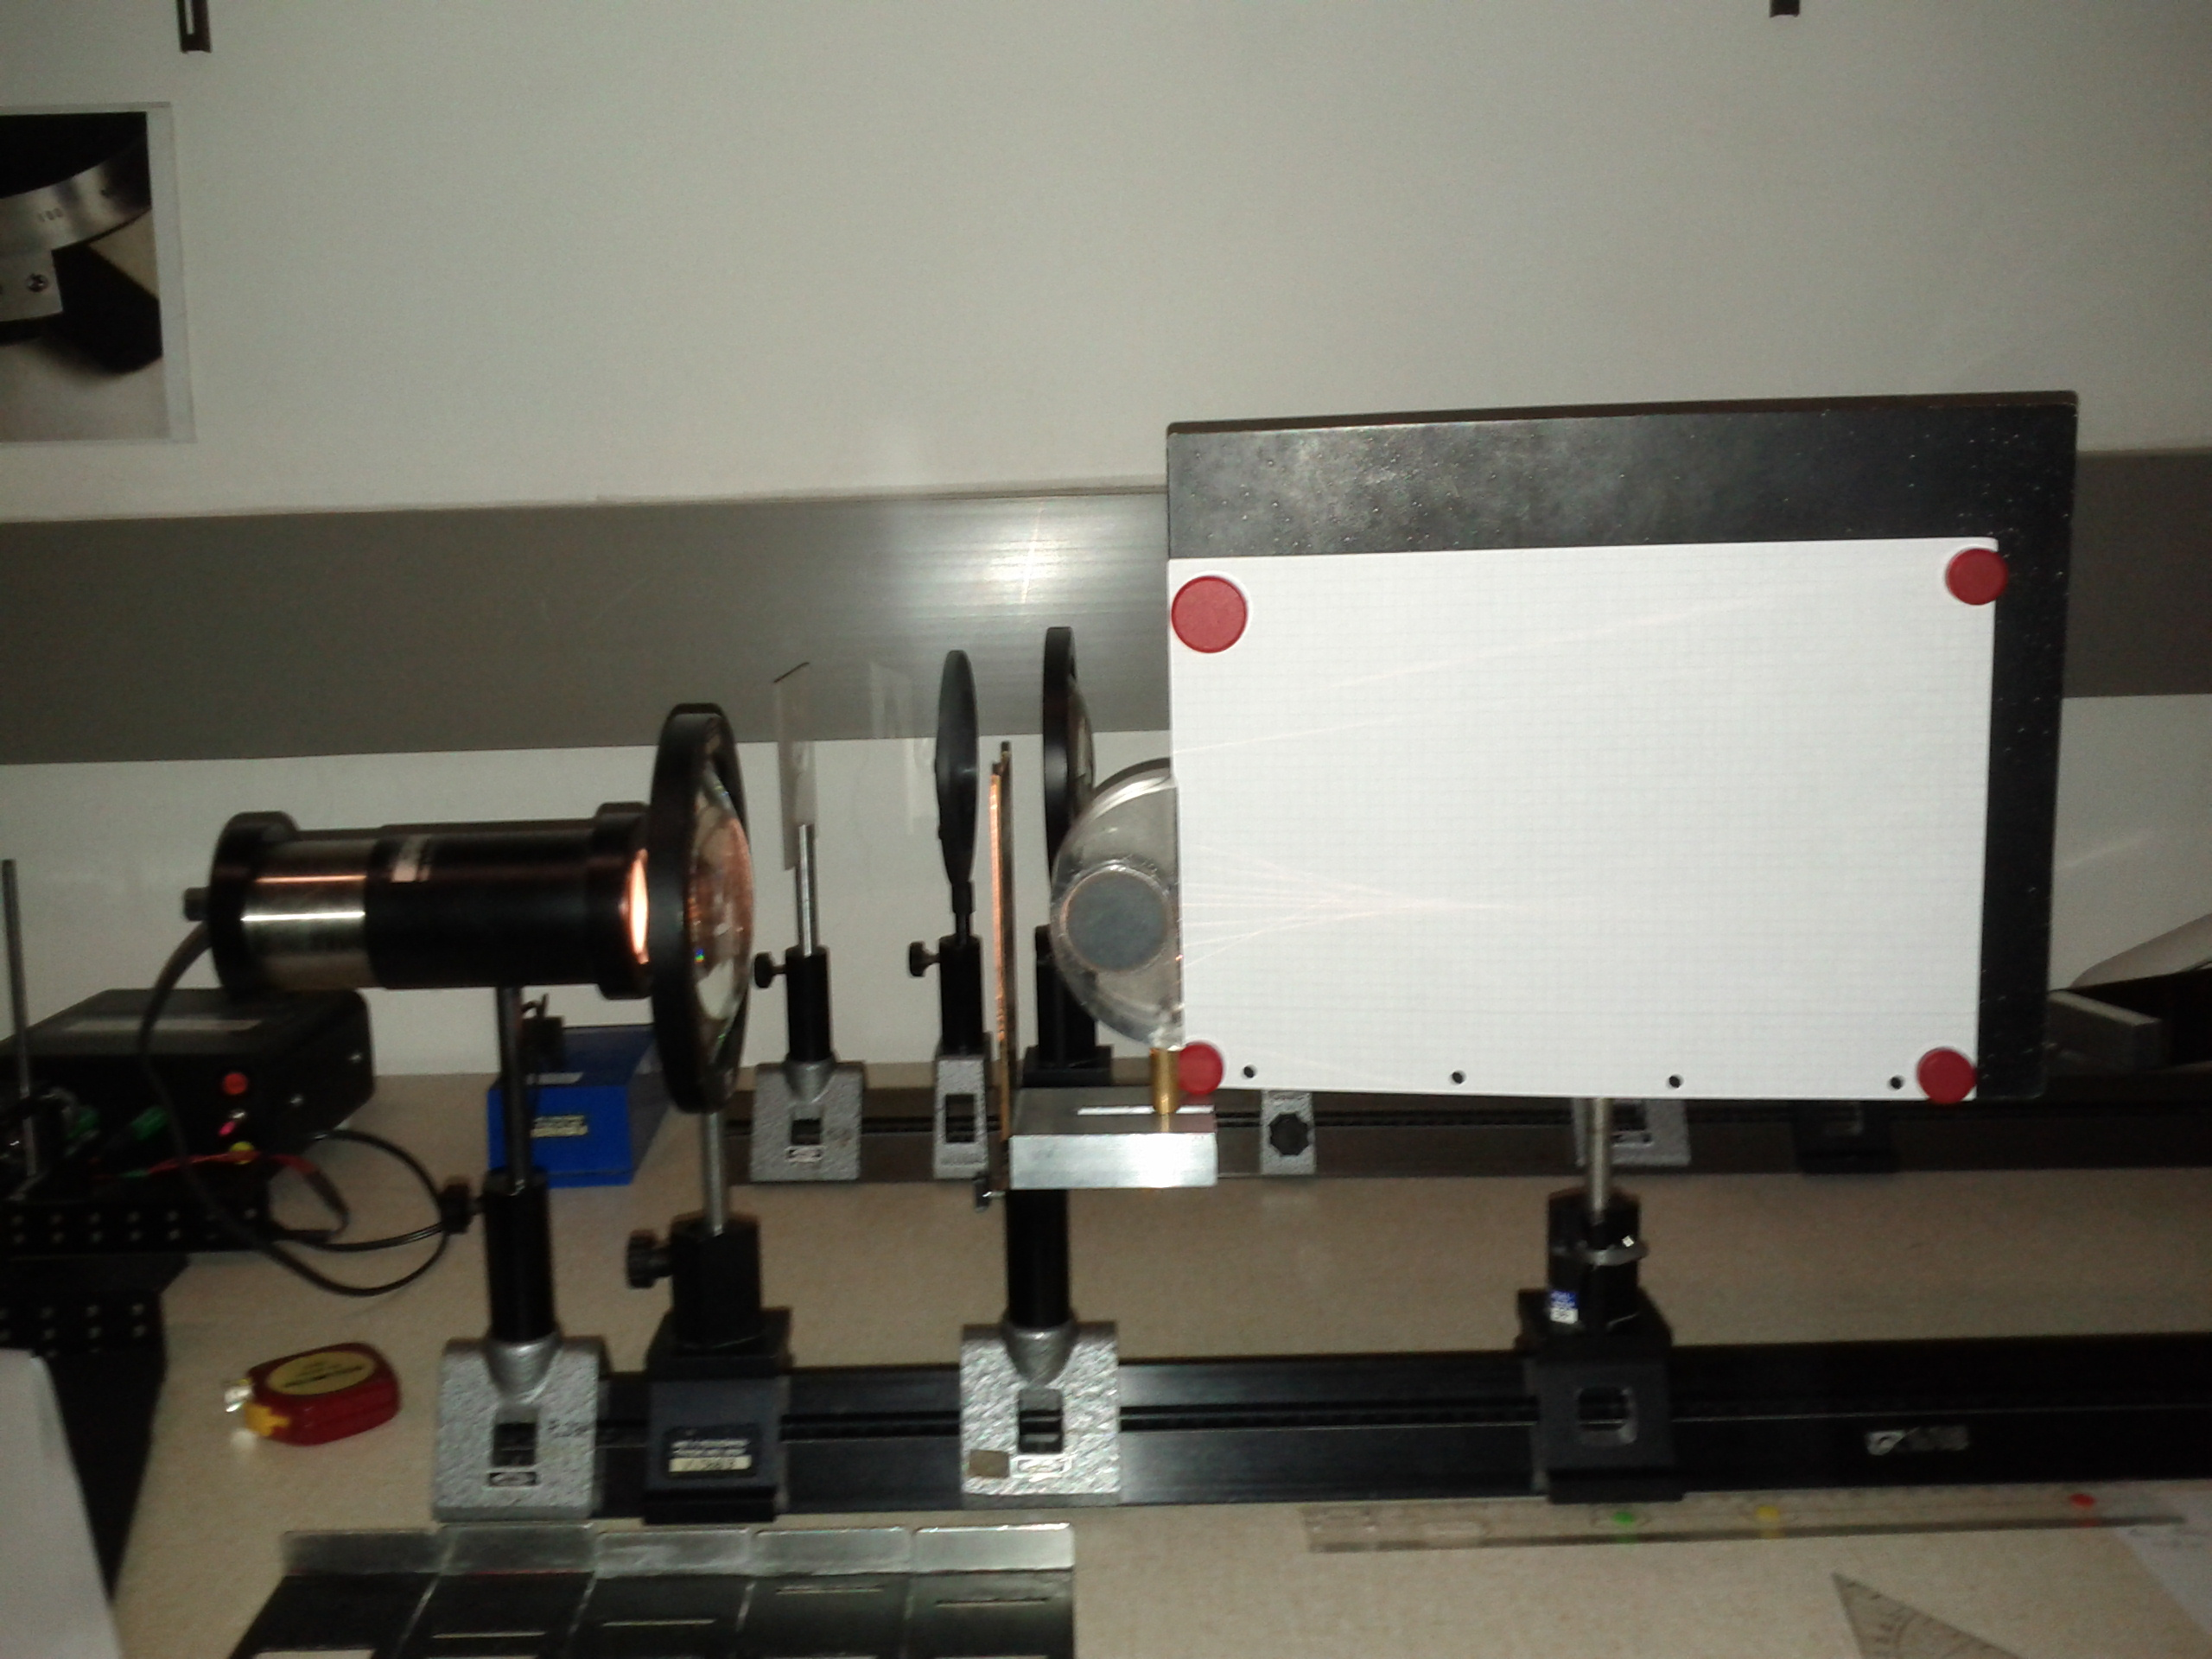
\includegraphics[scale=0.08]{./figure/linsenfehler.jpg}
	\caption{Versuchaufbau Plan-Konvex Linse}
	\label{fig:linsenfehler_aufbau}
\end{figure}
\subsection{Messwerte und Ergebnisse}

\end{multicols}
\pagebreak
\begin{figure}[H]
	\centering
	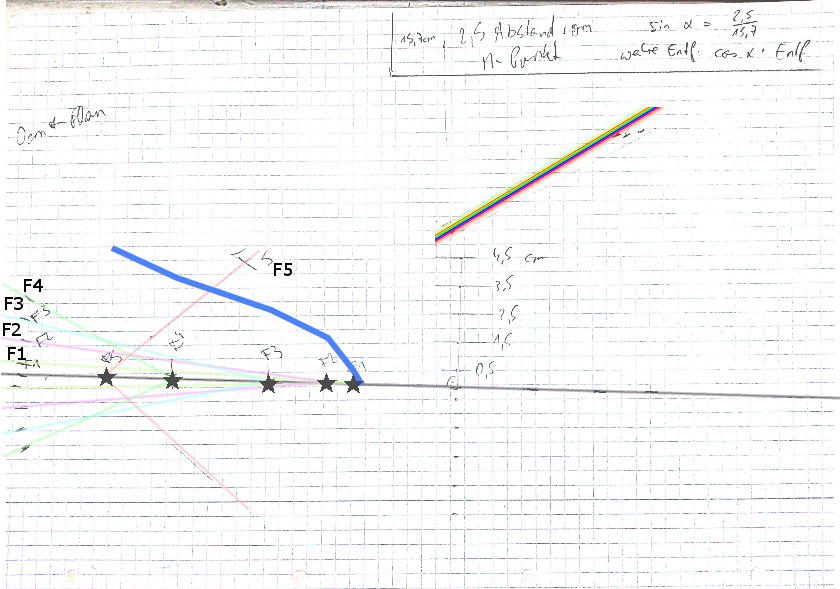
\includegraphics[scale=0.45]{./figure/konvex_plan.png}
	\caption{Linsenfehler Konvex-Plan Linse}
	\label{fig:linsenfehler_strahlen_konvex_plan}
\end{figure}
\noindent
\begin{figure}[H]
	\centering
	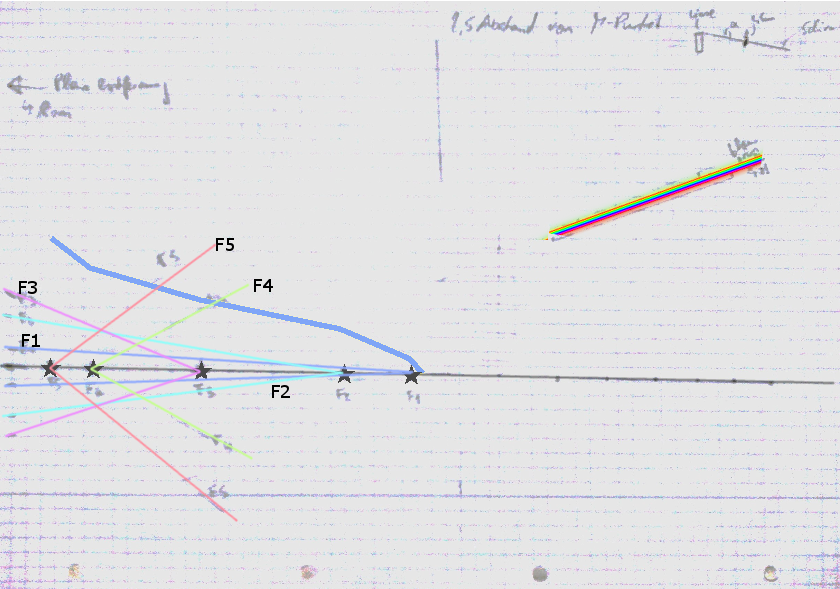
\includegraphics[scale=0.45]{./figure/plan_konvex.png}
	\caption{Linsenfehler Plan-Konvex Linse}
	\label{fig:linsenfehler_strahlen_plan_konvex}
\end{figure}
\pagebreak
\begin{multicols}{2}

\subsection{Diskussion}

%%%%%%%%%%%%%%%%%%%%%%%%%%%%%%%%%%%%
\section{Mikroskop}

In diesem Teil von PW6 soll ein (vereinfachtes) Mikroskop gebaut werden, und seine Vergrößerungseigenschaften sollen untersucht werden.\\
Es besteht aus einem vorgegebenen Rahmen mit Beleuchtung von unten, einem Objektträger (hier eine geeichte Strichplatte zur Längenmessung) und 2 Sammellinsen. Die Sammellinse mit der kleineren Brennweite dient als \textbf{Objektiv} und wird direkt über dem Objekt angebracht. Darüber, in einigem Abstand, wird die andere Linse als \textbf{Okular} montiert.\\
Die Distanz zwischen beiden Linsen beträgt mindestens die Summe der beiden Brennweiten. Die Länge, die darüber hinausgeht ist die \textbf{Tubuslänge $t$}.
Die Vergrößerung des Mikroskops ist gegeben durch:
$$V_M=\frac{t}{f_{Obj}}\frac{s_0}{f_{Ok}}$$
wobei $s_0=250mm$ der Abstand des Auges vom Standardnahpunkt ist.\\
Indem ein Maßstab außerhalb des Systems mit der Skala auf dem Objektträger verglichen wird, soll die Vergrößerung bei verschiedenen Tubuslängen experimentell festgestellt, wie auch berechnet werden.\\
Anschließend soll noch die Dicke eines Haares vermessen werden.

\begin{figure}[H]
	\centering
	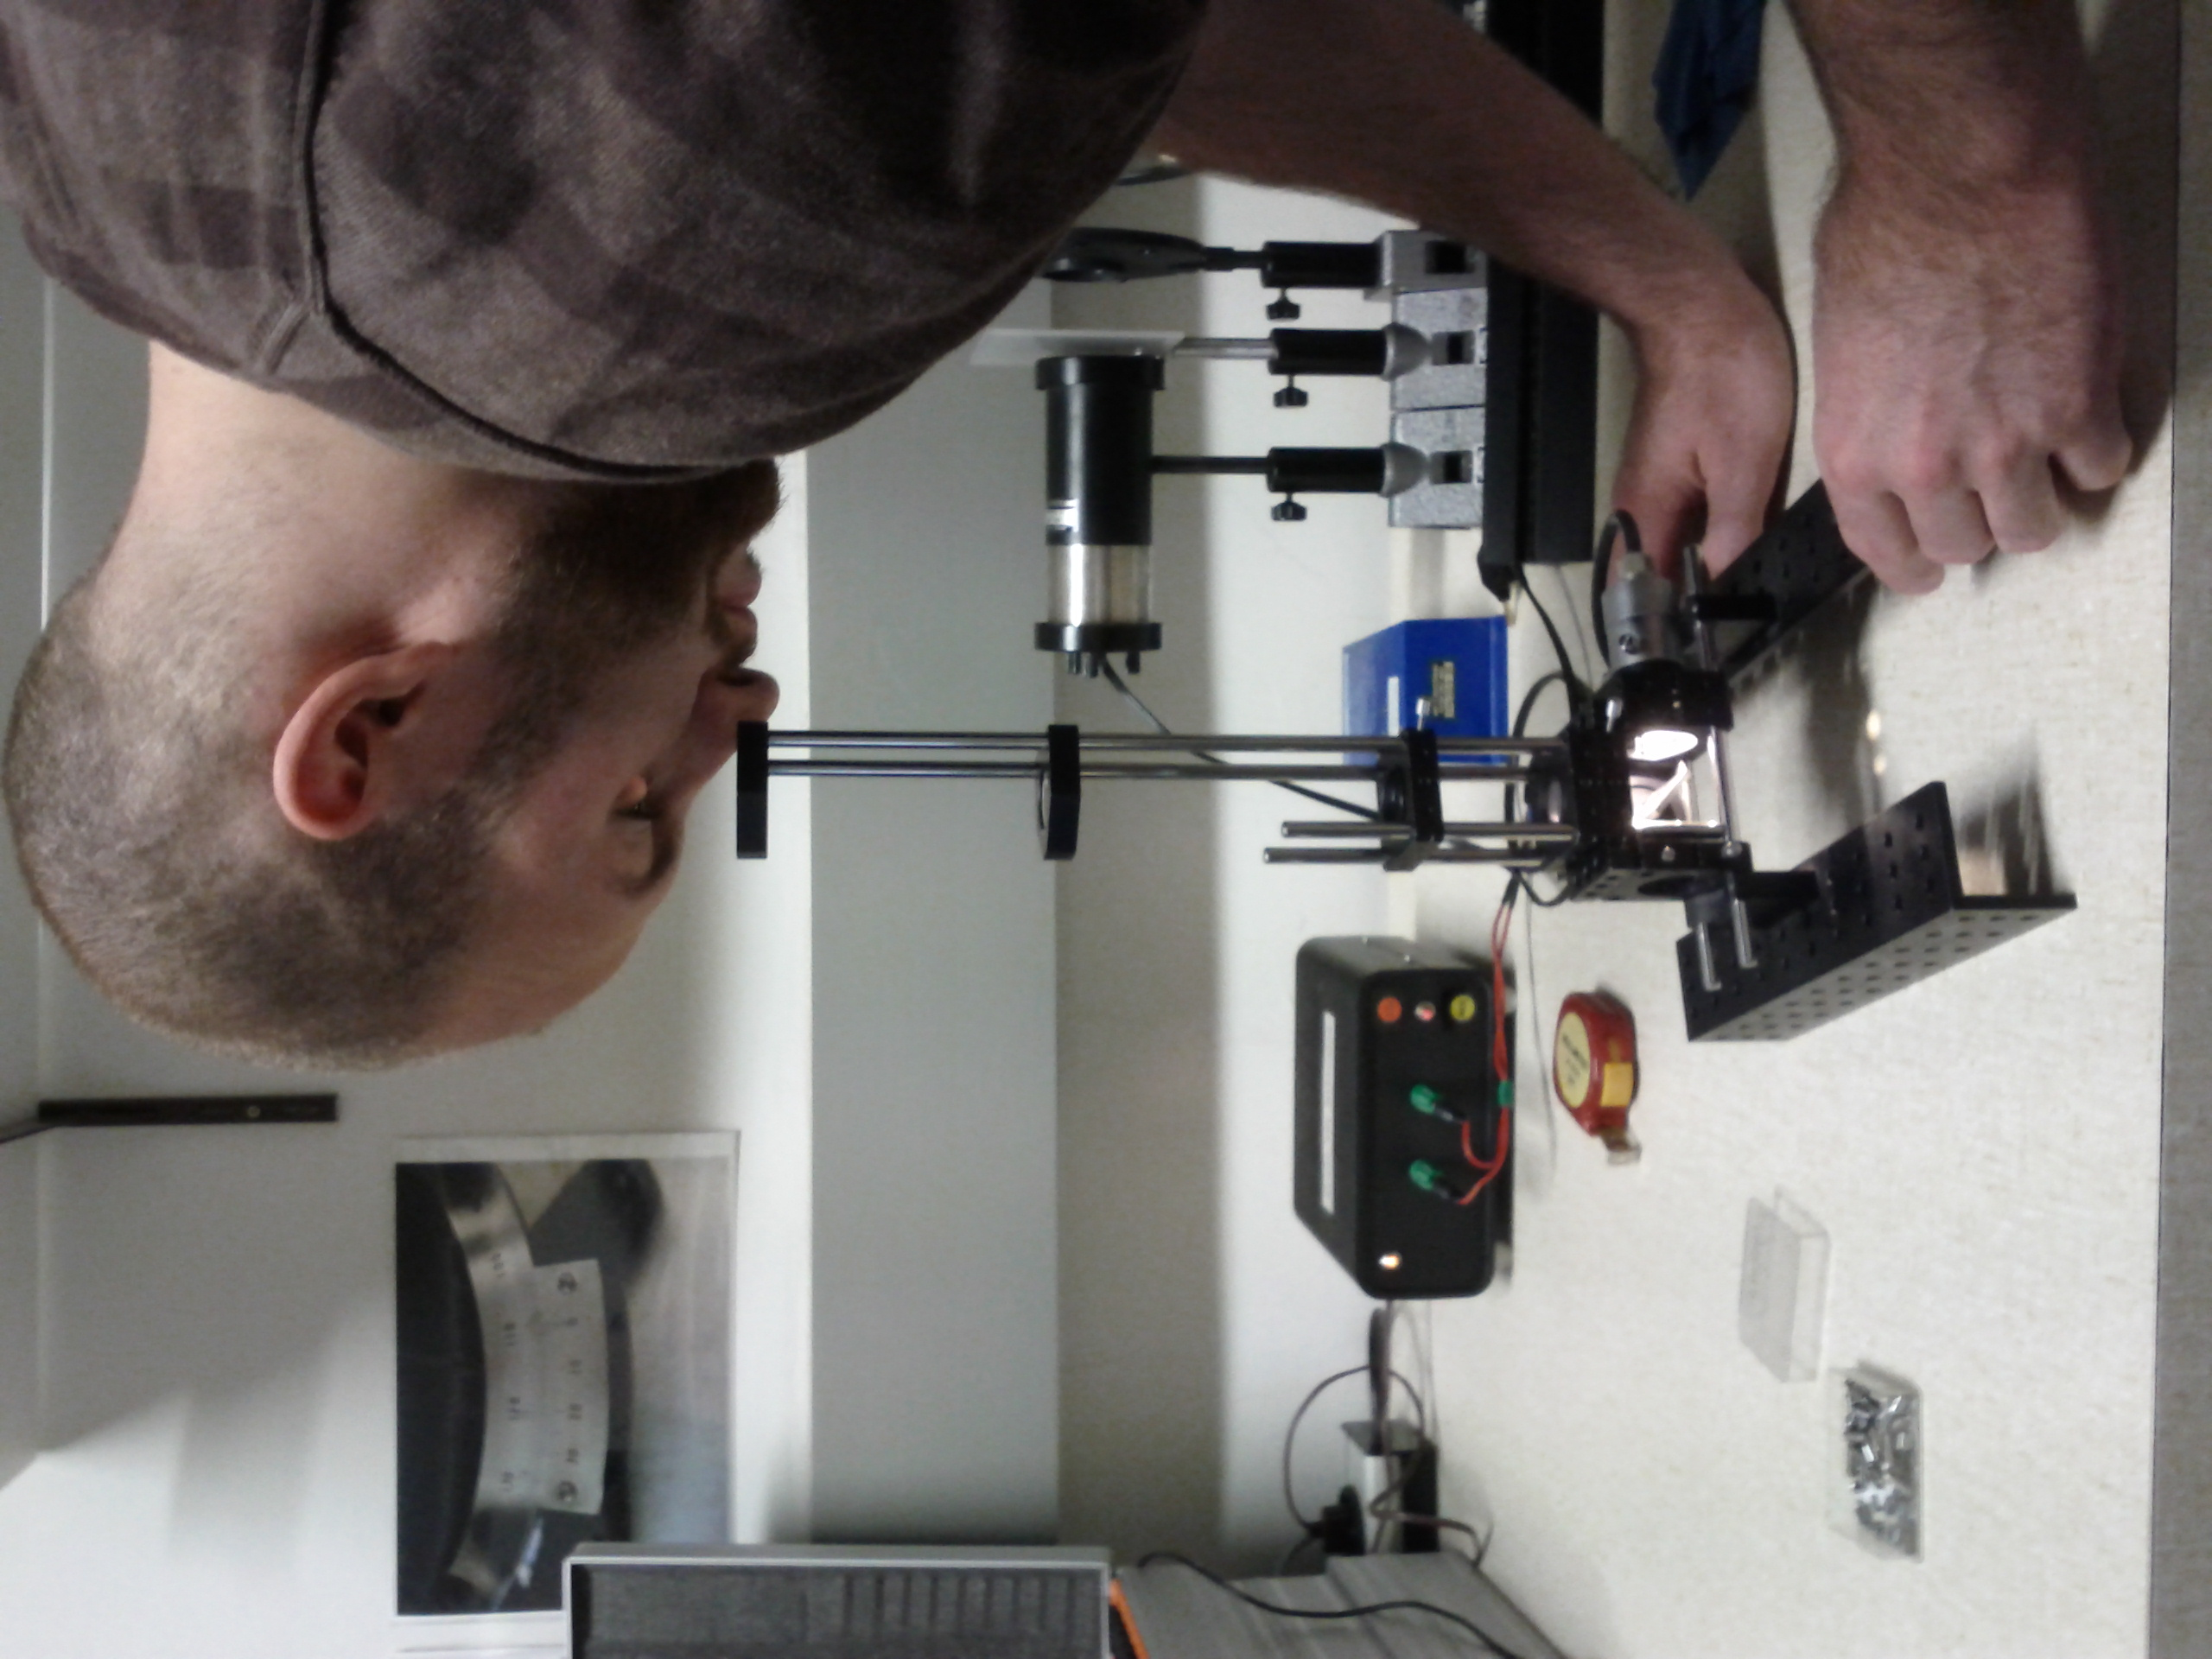
\includegraphics[angle=-90,scale=0.1]{./figure/mikroskop.jpg}
	\caption{Versuchaufbau Mikroskop mit Augenschutz}
	\label{fig:mikroskop_aufbau}
\end{figure}

\subsection{Messwerte und Ergebnisse}

Strichplatte: $10mm$ $\widehat{=}$ $200'$\\
Objektiv: $f_{Obj}=30mm$\\
Okular: $f_{Ok}=60mm$\\

\begin{itemize}

	\item 1. Tubus:\\
	$t_1=(30 \pm 1) mm$\\
	Messung:\\
	$60' \approx 10mm$\\
	\\
	$V_M= (3.3 \pm 1.0)fach$\\
	Rechnung: \\
	$V_M=(4.17\pm 0.14)fach$
	
	\item 2. Tubus:\\
	$t_2=(50 \pm 1) mm$\\
	Messung:\\
	$40' \approx 10mm$\\
	\\
	$V_M= (5.0 \pm 1.5)fach$\\
	Rechnung: \\
	$V_M=(6.94 \pm 0.14)fach$
	
	\item 3. Tubus:\\
	$t_3=(80 \pm 1) mm$\\
	Messung:\\
	$20' \approx 12mm$\\
	\\
	$V_M= (12.0 \pm 3.0)fach$\\
	Rechnung: \\
	$V_M=(11.11 \pm 0.14)fach$
	
	\item 34. Tubus:\\
	$t_4=(65 \pm 1) mm$\\
	Messung:\\
	$20' \approx 10mm$\\
	\\
	$V_M= (10.0 \pm 3.0)fach$\\
	Rechnung: \\
	$V_M=(9.03 \pm 0.14)fach$
	
	
\end{itemize}

\noindent Vermessung eines \textbf{Haares}:\\
\textit{(courtesy of Johanna Akbarzadeh)}\\
Tubuslänge $t= (80 \pm 1)mm$\\
Dicke des Haares: $(2 \pm 1)'$\\
$$d_{Haar} = (0.10 \pm 0.05)mm$$



\subsection{Diskussion}

Dieser einfache Aufbau liefert die erwarteten Ergebnisse. Dabei ist - im Vergleich von Messung und Rechnung - vor allem auch die Ungenauigkeit der Methode gut zu erkennen, bzw. ihre Abhängigkeit vom Geschick der Augenmuskulatur und Sehkraft.\\
Beide Experimentierenden weisen hier Defizite auf (nach Gesprächen im Aufenthaltsraum, dürfte es durchaus KollegInnen geben, denen dieses Experiment genauer gelungen ist).\\
Daher wurde im Vergleich eines Maßstabes mit der Skala im Mikroskop eine vergleichsweise große Unsicherheit von $\pm 3mm$ für alle Messungen angenommen. Vor allem Tubuslänge $t_1$ und $t_2$ zeigen, dass dies notwendig ist, wobei das gerechnete Ergebnis für  $V_M(t_2)$ sogar außerhalb des abgeschätzten Unsicherheitsbereiches liegt.\\
Die Versuche 1 und 2 aus PW6 haben zwar gezeigt, dass auch die verwendeten Linsen durchaus deutliche Abweichungen haben könnten, aufgrund der Erfahrung aus der Durchführung dieses Experimentes sind jedoch wohl menschliche Ungenauigkeiten die Hauptursache für die groben Ergebnisse.\\
Es wurden verschiedene Positionen für den äußeren Maßstab versucht, letztendlich ist aber das gleichzeitige betrachten 2er Systeme mit 2 Augen eine, für uns zumindest, außerordentlich schwierige Methode, und vor allem als Lehrbeispiel geeignet.\\
Der lineare Zusammenhang zwischen Tubuslänge und Vergrößerung, der aus der Rechnung deutlich hervorgeht, ist mit diesem Experiment nicht bestätigt: Während für $t_1$ und $t_2$ das gemessene Ergebnis niedriger ausfällt, als das erwartete, liegen die Vergrößerungen bei $t_3$ und $t_4$ höher.\\
Nachdem aber damit zu rechnen ist, dass die Verzerrungen vor allem aus den groben Abschätzungen stammen, lässt sich keinesfalls aus den Ergebnissen darauf schließen, dass der lineare Zusammenhang aus der Rechnung falsch sei.\\
\\
Mit einem großen Unsicherheitsbereich liegt auch die Dicke des Haares innerhalb der Erwartung.\\
Der Wikipedia-Artikel über das menschliche Haar gibt dessen Dicke mit bis zu $0.12mm$ für das Haupthaar an.\\
\\
Eine leichte Verbesserung des Aufbaus ergab sich durch das montieren einer dritten Linsenfassung, ohne Linse, ursprünglich als Schutz vor den Führungsstangen. Die zusätzliche Stabilität durch das Anlehnen der Augenpartie, hat dabei ein deutlich stabileres Ablesen erst ermöglicht.

%%%%%%%%%%%%%%%%%%%%%%%%%%%%%%%%%%%%
\section{Fernrohr}
In diesem versuch werden 2 einfache Fernrohre gebaut und deren errechnete Vergrößerung an einer Skala in ein paar m Entfernung überprüft.\\
Das astronomische Fernrohr besteht aus 2 Sammellinsen. Ihr Abstand ist genau die Summe beider Brennweiten, wobei das erzeugt Bild umgekehrt ist. Für kleine Sehwinkel, wie bei einem Fernrohr der Fall, gelten gleiche Verhältnisse für die Winkel der Mittelpunktsstrahlen zum Bild zwischen den Linsen, und den Quotienten aus Abbildung und Brennweiten:
$$V_f=\frac{\epsilon}{\epsilon_1}=\frac{f_{obj}}{f_{ok}}$$
Das holländische Fernrohr hat als Okular eine Zerstreuungslinse und liefert damit ein richtig orientiertes Bild. Der Abstand zwischen den Linsen ist hier die Differenz der Brennweitenbeträge.

\subsection{Messwerte und Ergebnisse}
Objektiv (Sammellinse): $f_{obj}=60mm$\\
Okulare:\\
astronomisches: $f_{ok}=30mm$\\
holländisches: $f_{ok}=40mm$\\
\\
\textbf{astronomisches Fernrohr:}\\
Messung Braun: $3'_{FR} \widehat{=} 6'_{real}\Rightarrow V_F=2 fach$\\
Messung Kurz: $2'_{FR} \widehat{=} 4'_{real}\Rightarrow V_F=2 fach$\\
\\
Rechnung: $V_F = \frac{60}{30}=2fach$\\
\\
\textbf{astronomisches Fernrohr:}\\
Messg Braun: $3'_{FR} \widehat{=} 2'_{real}\Rightarrow V_F=1.5fach$\\
Messg Kurz: $1.5'_{FR} \widehat{=} 1'_{real}\Rightarrow V_F=1.5fach$\\
\\
Rechnung: $V_F = \frac{40}{30}=1.33fach$\\




\subsection{Diskussion}

Ähnlich dem Mikroskop-Versuch,  gestaltet sich auch hier der Vergleich zwischen einem realen und einem vergrößerten Maßstab, jeweils mit einem Auge, als schwierig. Es ist unmittelbar aus dem Experiment klar, dass die Messung sehr ungenau ist.\\
Eine realistische Abschätzung der Unsicherheit wäre wohl etwa ein halber Streifen an der Tafel. Bei einem Vergleich mit wenigen Streifen (zB. Kurz, astronomisches Fernrohr) führt das zu einer Unsicherheit der Vergrößerung von bis zu 50\%.\\
Diese Methode erweist sich also (zumindest unter den gegebenen Bedingungen und Fähigkeiten) als sehr ungenau.\\
Dennoch stimmen die Ergebnisse mit der Rechnung überein (auch wenn für das holländische Fernrohr die Erwartungshaltung nach einem möglichst klaren Ergebnis wohl bei beiden Experimentierenden zu einem Bias geführt hat).\\
\\
Die theoretische Berechnung der Vergrößerungen gilt für kleine Sehwinkel, da die Kleinwinkel-Näherung des Tangens verwendet wird.\\
Es ist jedoch davon auszugehen, dass diese Näherung bei Weitem genauer ist, als die Bestimmung der Vergrößerung durch die Augen.\\
(Leider wurde die Entfernung des Fernrohrs zur Wand und die höhe der Tafel nicht gemessen, aber selbst für eine grobe Schätzung trifft die Kleinwinkel-Näherung gut zu:
$$\frac{1m}{4m}=0.25\approx 0.245= \arctan (\frac{1m}{4m})$$

\section{Quellen}
$[1]$ Leitfaden, \url{http://www.univie.ac.at/anfpra/neu1/pw/pw6/PW6PL4.pdf}\\
$[2]$ Haaresbreite: \url{http://de.wikipedia.org/wiki/Haar}

\end{multicols}
\end{document}